\documentclass[11pt]{beamer}
\usepackage{booktabs}
\usepackage{array}
\usepackage{eulervm}
% \usepackage{fontspec}
\usepackage[scaled]{helvet}
% \usepackage{lmodern}
\usepackage[T1]{fontenc}

\newcommand{\gap}{\vspace{0.8em}}
% \setmonofont[Path=./fonts/,Scale=0.9]{JetBrainsMono.ttf}
% \setmainfont[Path=./fonts/]{KingsBureauGrot-FiveOne.ttf}
% \setsansfont{Fira Sans}
% \setsansfont{IBM Plex Sans}

% \setmonofont[Path=./fonts/,Scale=0.9]{JetBrainsMono.ttf}
% \setmainfont[Path=./fonts/]{KingsBureauGrot-FiveOne.ttf}
% \setsansfont[Path=./fonts/]{KingsCaslon.ttf}
% \setsansfont{IBM Plex Sans}
% \setbeamerfont{title page}{family=\rmfamily}
% \setbeamerfont{frametitle}{family=\rmfamily}

% References ------------------------------------------------------------------

\usepackage[%
  backend     = bibtex,
  style       = numeric,
  sorting     = ynt,
  sortcites   = true,
  autocite    = superscript
]{biblatex}

\addbibresource{references.bib}

% tcolorbox -------------------------------------------------------------------

\usepackage{tcolorbox}
\newtcolorbox{cbox}[3][]
{
  colframe = #2!10,
  colback  = #2!10,
  coltitle = #2,  
  colbacktitle = #2!10,
  lefttitle = 1mm,
  toptitle = 1mm,
  colupper = #2,  
  title    = {#3},
  fonttitle = \bfseries,
  #1,
  arc=0.2mm,
  left=1mm,
  before upper={\setbeamercolor{item}{fg=#2}},
  after upper={\setbeamercolor{item}{fg=#2}}
}

\usepackage{graphicx}
\newcommand*{\img}[1]{%
    \raisebox{-.3\baselineskip}{%
        \includegraphics[
        height=\baselineskip,
        width=\baselineskip,
        keepaspectratio,
        ]{#1}%
    }%
}

\title[The \texttt{pmsims} package for R]{
    A simulation approach to calculating minimum sample sizes for prediction modelling
}
\subtitle{The \texttt{pmsims} package for R}
\date{29$^{\text{th}}$ August 2023}
\author[Biostatistics \& Health Informatics, KCL]{%
    Ewan Carr, Gordon Forbes, Diana Shamsutdinova, Daniel Stahl, 
    and Felix Zimmer}
\institute[]{Department of Biostatistics \& Health Informatics\\ King's College London}
\titlegraphic{
\includegraphics[height=1.5cm]{figures/kcl.png}}
\setbeamertemplate{navigation symbols}{}
\setbeamertemplate{footline}[frame number]

% Theme
\definecolor{KCLpurple}{RGB}{80, 20, 145}
\definecolor{KCLred}{RGB}{226, 35, 26}
\definecolor{KCLhotpink}{RGB}{200, 50, 150}
\definecolor{KCLpurple}{RGB}{80, 20, 145}
\definecolor{KCLseablue}{RGB}{0, 90, 210}
\definecolor{KCLtealblue}{RGB}{0, 154, 166}
\usecolortheme[named=KCLseablue]{structure}
\setbeamercolor{alerted text}{fg=KCLhotpink}

\setbeamertemplate{itemize items}[circle]
\setbeamertemplate{enumerate items}[default]

\newenvironment{itemize*}%
{\begin{itemize}%
		\setlength{\itemsep}{100pt}%
		\setlength{\parskip}{0pt}}%
		{\end{itemize}}

\begin{document}

\maketitle

\section{Introduction}

\begin{frame}{30-second version}
	\Large
	\begin{enumerate}
		\setlength{\itemsep}{12pt}

		\item Prediction models developed with inadequate samples lead to
		      \alert{overfitting} and \alert{imprecise} estimates.

		\item Existing tools use \alert{analytical methods} to derive minimum
		      samples sizes for continuous, binary, and survival outcomes.

		\item We've developed a \alert{simulation-based} approach that can
		      be applied to \alert{any} outcome or method.
	\end{enumerate}
\end{frame}

\begin{frame}[c]
	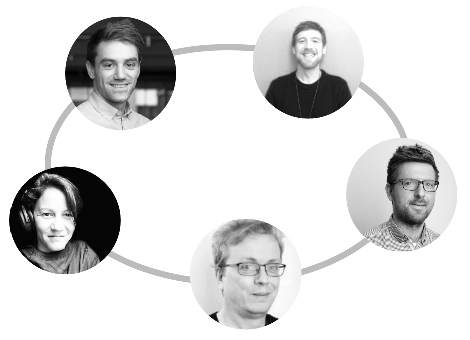
\includegraphics[width=\textwidth]{figures/group_photos.pdf}
\end{frame}

\begin{frame}[t]{Overview}
	\begin{enumerate}
		\item Background
		      \begin{itemize}
			      \item What's the problem?
			      \item What solutions already exist?
		      \end{itemize}
		\item Our approach
		      \begin{itemize}
			      \item Simulation to identify minimum sample size that satisfies criteria.
			      \item Flexible, but slower.
			      \item Gaussian process regression (via \texttt{mlpwr}) to speed up.
		      \end{itemize}
		\item Next steps
	\end{enumerate}
\end{frame}

\section{Background}

\begin{frame}[t]{What's the problem?}

	\begin{itemize}
		\item Thousands of prediction models are developed every year.
		\item Prediction models can inform treatment decisions, facilitate
		      screening, and enable stratified care.
		\item  However, most are developed with inadequate samples.
	\end{itemize}

	\begin{cbox}{KCLtealblue}{}
		\begin{itemize}
			\item In a review of prediction models for COVID-19, the most
			      frequent problem was insufficient sample size. 67\%
			      (408/731) of models were developed on too few
			      patients\autocite{wynants2020}.
			\item 56\% of models developed using supervised machine learning
			      techniques are developed using inadequate sample
			      sizes\autocite{navarro2021}.
			\item 73\% of prediction models for psychiatry had inadequate
			      sample size\autocite{meehan2022}.
			\item 8\% of machine learning models published in oncology report a
			      sample size justification\autocite{dhiman2022}.
		\end{itemize}
	\end{cbox}
\end{frame}

\begin{frame}[t]{Inadequate samples $\rightarrow$ research waste}

	\begin{itemize}
		\item Inadequate samples lead to overfitting and inaccurate estimates
		      of model parameters.
		      \begin{itemize}
			      \item Overfitting is where the model captures idiosyncrasies
			            of the development sample, producing inflated
			            estimates of predictive performance that cannot be
			            replicated in the target population.
		      \end{itemize}
		\item Unreliable models may generate inappropriate decisions about
		      patient care or lead to models not being implemented into
		      clinical practice.
		\item Data collection can be invasive and inconvenient and diverts
		      resources from other activities that benefit patients.

	\end{itemize}

	\begin{cbox}{KCLseablue}{}
		Ensuring sample sizes are sufficient \emph{before model development}
		would improve patient outcomes by avoiding models developed with
		inadequate samples and reducing participant burden.
	\end{cbox}

\end{frame}

\begin{frame}[t]{Tools for estimating minimum sample sizes for prediction}

	Until recently, most studies ignored sample size.

	Or they used simple rules-of-thumb (e.g., 10 events per variable).

	In 2018, \texttt{pmsampsize} was released by Riley et al.

	\begin{columns}
		\begin{column}[c]{0.5\textwidth}
			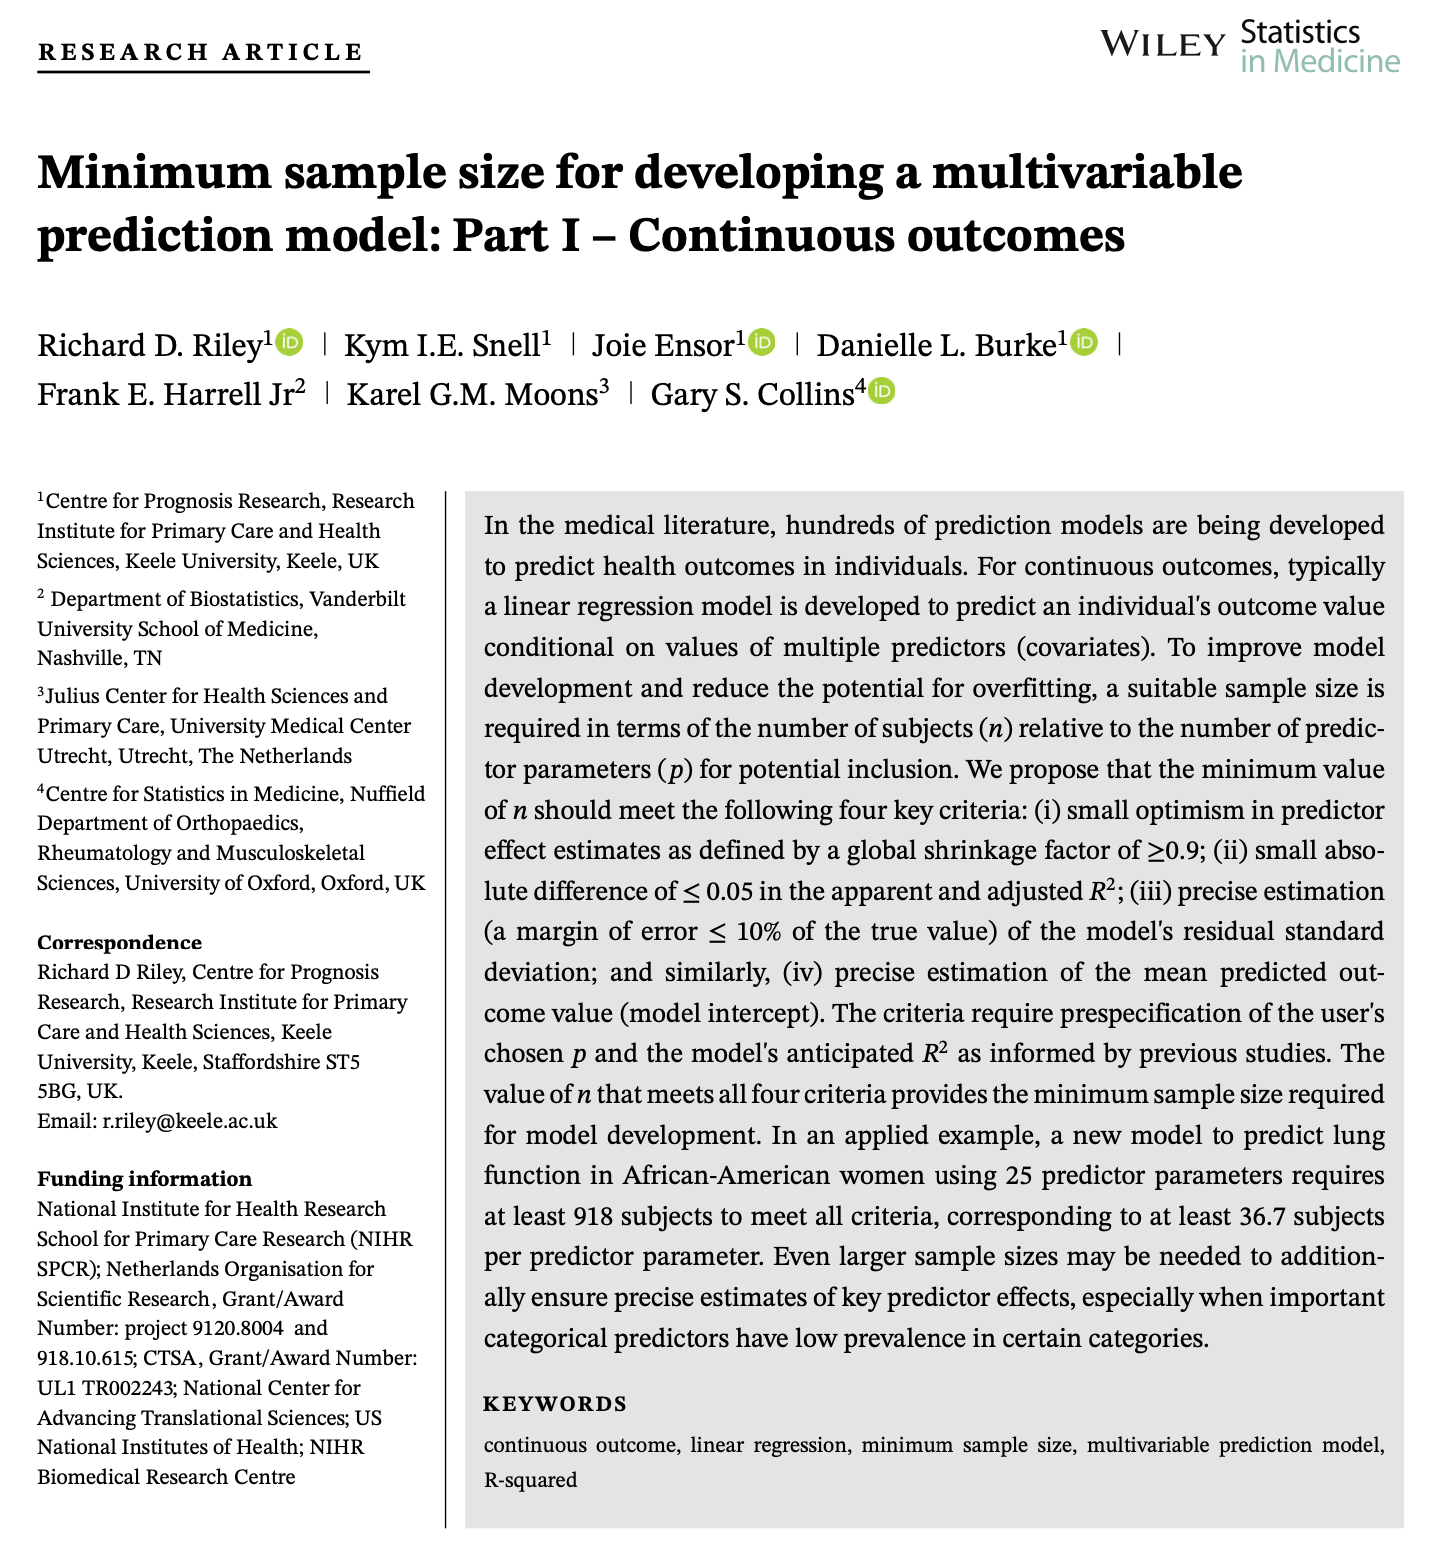
\includegraphics[width=\textwidth]{figures/riley1.png}

		\end{column}
		\begin{column}[c]{0.5\textwidth}
			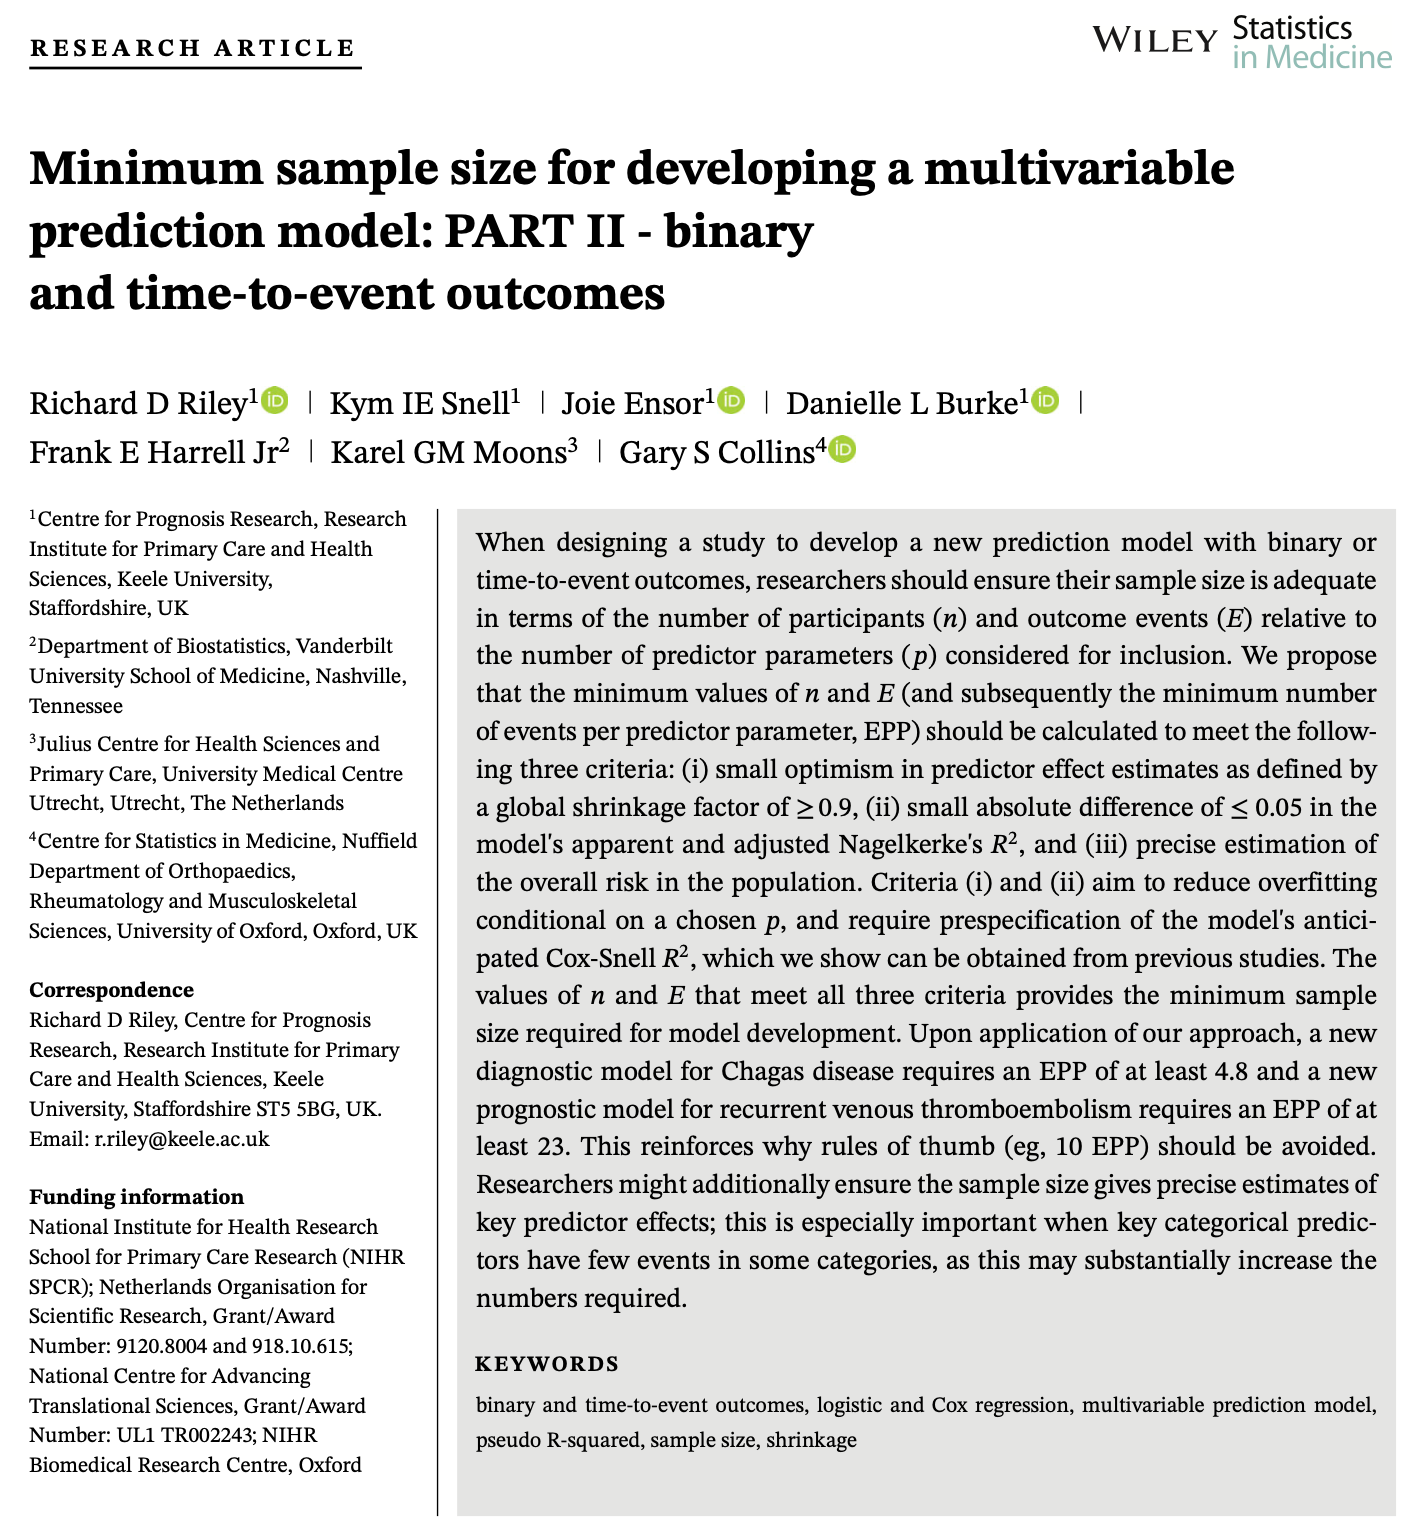
\includegraphics[width=\textwidth]{figures/riley2.png}

		\end{column}
	\end{columns}

\end{frame}

\begin{frame}{pmsampsize}

	The package identifies the minimum sample that results in: \\[1em]

	\centering

	\begin{tabular}{l>{\raggedright\arraybackslash}p{12em}>{\raggedright\arraybackslash}p{12em}}
		           & \textbf{Continuous}                                          & \textbf{Binary} \\ \midrule
		i.         & \multicolumn{2}{p{24em}}{Small optimism in predictor effect
		estimates, indicated by a global shrinkage factor of ≥ 0.9.}                                \\ \midrule
		ii.        & \multicolumn{2}{p{20em}}{Small absolute difference of ≤ 0.05
		in the apparent and adjusted $R^2$}                                                         \\ \midrule
		iii.       & Precise estimation of the model's residual standard
		deviation. & Precise estimation of the overall risk in the
		population.                                                                                 \\ \midrule
		iv.        & Precise estimation of the model intercept.                   &                 \\
	\end{tabular}

\end{frame}

\begin{frame}[t]{We \img{figures/heart.png} pmsampsize, however\ldots}

	pmsampsize has methods for simple continuous, binary, and survival
	outcome. However, we increasingly need to derive minimum samples for:\

	\begin{cbox}{KCLtealblue}{Other types of model}
		e.g., machine learning algorithms such as random forests or gradient boosting.
	\end{cbox}

	\begin{cbox}{KCLhotpink}{Other data types}{}
		e.g., repeated measures and longitudinal data.
	\end{cbox}

	So, we've created a simulation-based framework for sample size estimation
	for prediction.

\end{frame}

\begin{frame}{pmsims}

	A simulation-based framework that derives the minimum sample that
	achieves:

	\begin{itemize}
		\item Within 10\% of the expected large-sample performance;
		\item Calibration slope of >0.9
	\end{itemize}

	\gap

	Key features:

	\begin{itemize}
		\item Can be used with any model or data type
		\item Provides defaults for common model and data types
		\item Efficient
	\end{itemize}

	\gap
	An R package.

\end{frame}

\begin{frame}[c]{Our approach}

    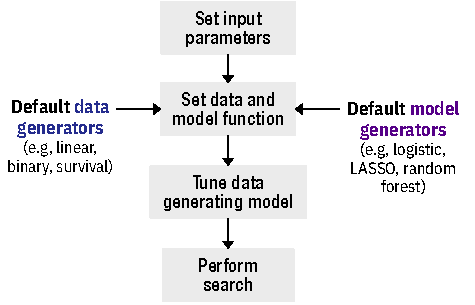
\includegraphics[width=\textwidth]{figures/workflow1.pdf}

\end{frame}

\begin{frame}[t]{Slide explaining input parameters}

	\begin{itemize}
		\item \texttt{simulate\_continuous}
		\item \texttt{simulate\_binary}
		\item \texttt{simulate\_survival}
	\end{itemize}

	Which each call:

	\begin{itemize}
		\item \texttt{simulate\_custom}
	\end{itemize}

\end{frame}

\begin{frame}[t]{Slide explaining default data and model generators}

    List default data/model/metrics.

\end{frame}

\begin{frame}{Performing the search:\ \texttt{mlpwr}}

	\begin{cbox}{KCLpurple}{}
		A simulation-based approach with complex data or models would be too
		slow.
	\end{cbox}

	\begin{columns}
		\begin{column}[c]{0.5\textwidth}
			\texttt{mlpwr} is a R package by Felix Zimmer and Rudolf Debelak at
			the University of Zurich.
			\begin{quote}
				``A Power Analysis Toolbox to Find Cost-Efficient Study Designs''
			\end{quote}
		\end{column}
		\begin{column}[c]{0.5\textwidth}
			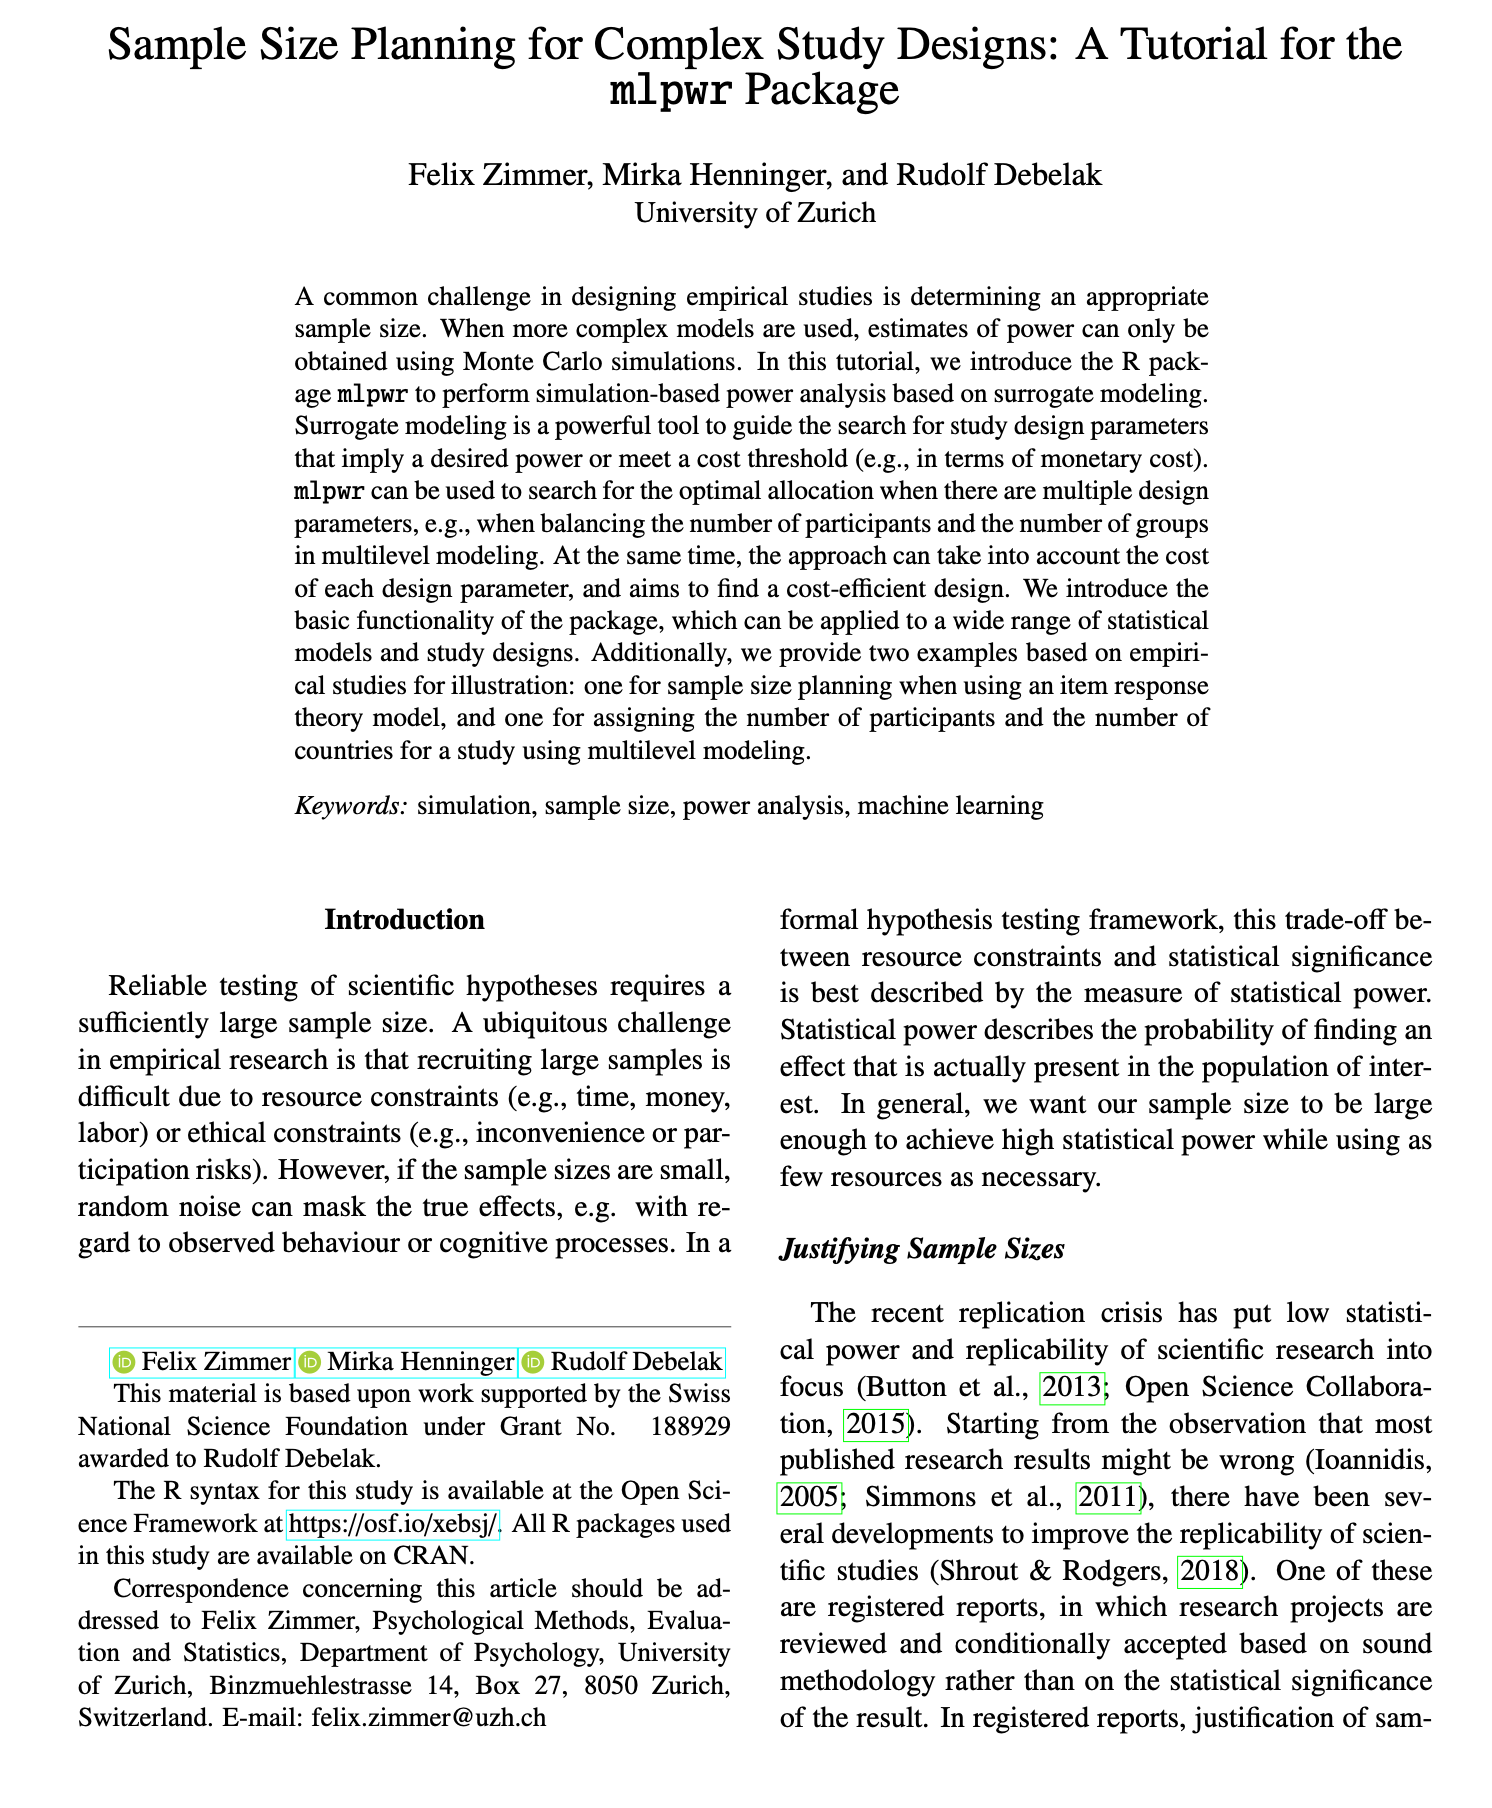
\includegraphics[width=\textwidth]{figures/mlpwr_paper.png}
		\end{column}
	\end{columns}

\end{frame}

\begin{frame}[t]{Surrogate modeling}

	\begin{itemize}
		\item Surrogate modeling aims to approximate a relationship that is
		      costly to investigate with a cheaper function (Bhosekar &
		      Ierapetritou, 2018; Forrester & Keane, 2009).

		\item  We can adopt the idea of surrogate modeling to the functional
		      relationship between study design parameters and power.

		\item Using this functional relationship, we can predict the power for
		      a sample size that we did not perform a simulation at
		      beforehand.

		\item Surrogate modeling is more efficient than grid search: In a
		      simple example, our approach required only 20\% of the
		      computational effort and performed 50\% more simulation runs
		      that used the optimal sample size (Zimmer \& Debelak, 2022).

	\end{itemize}

\end{frame}

\begin{frame}[c]{Example}

    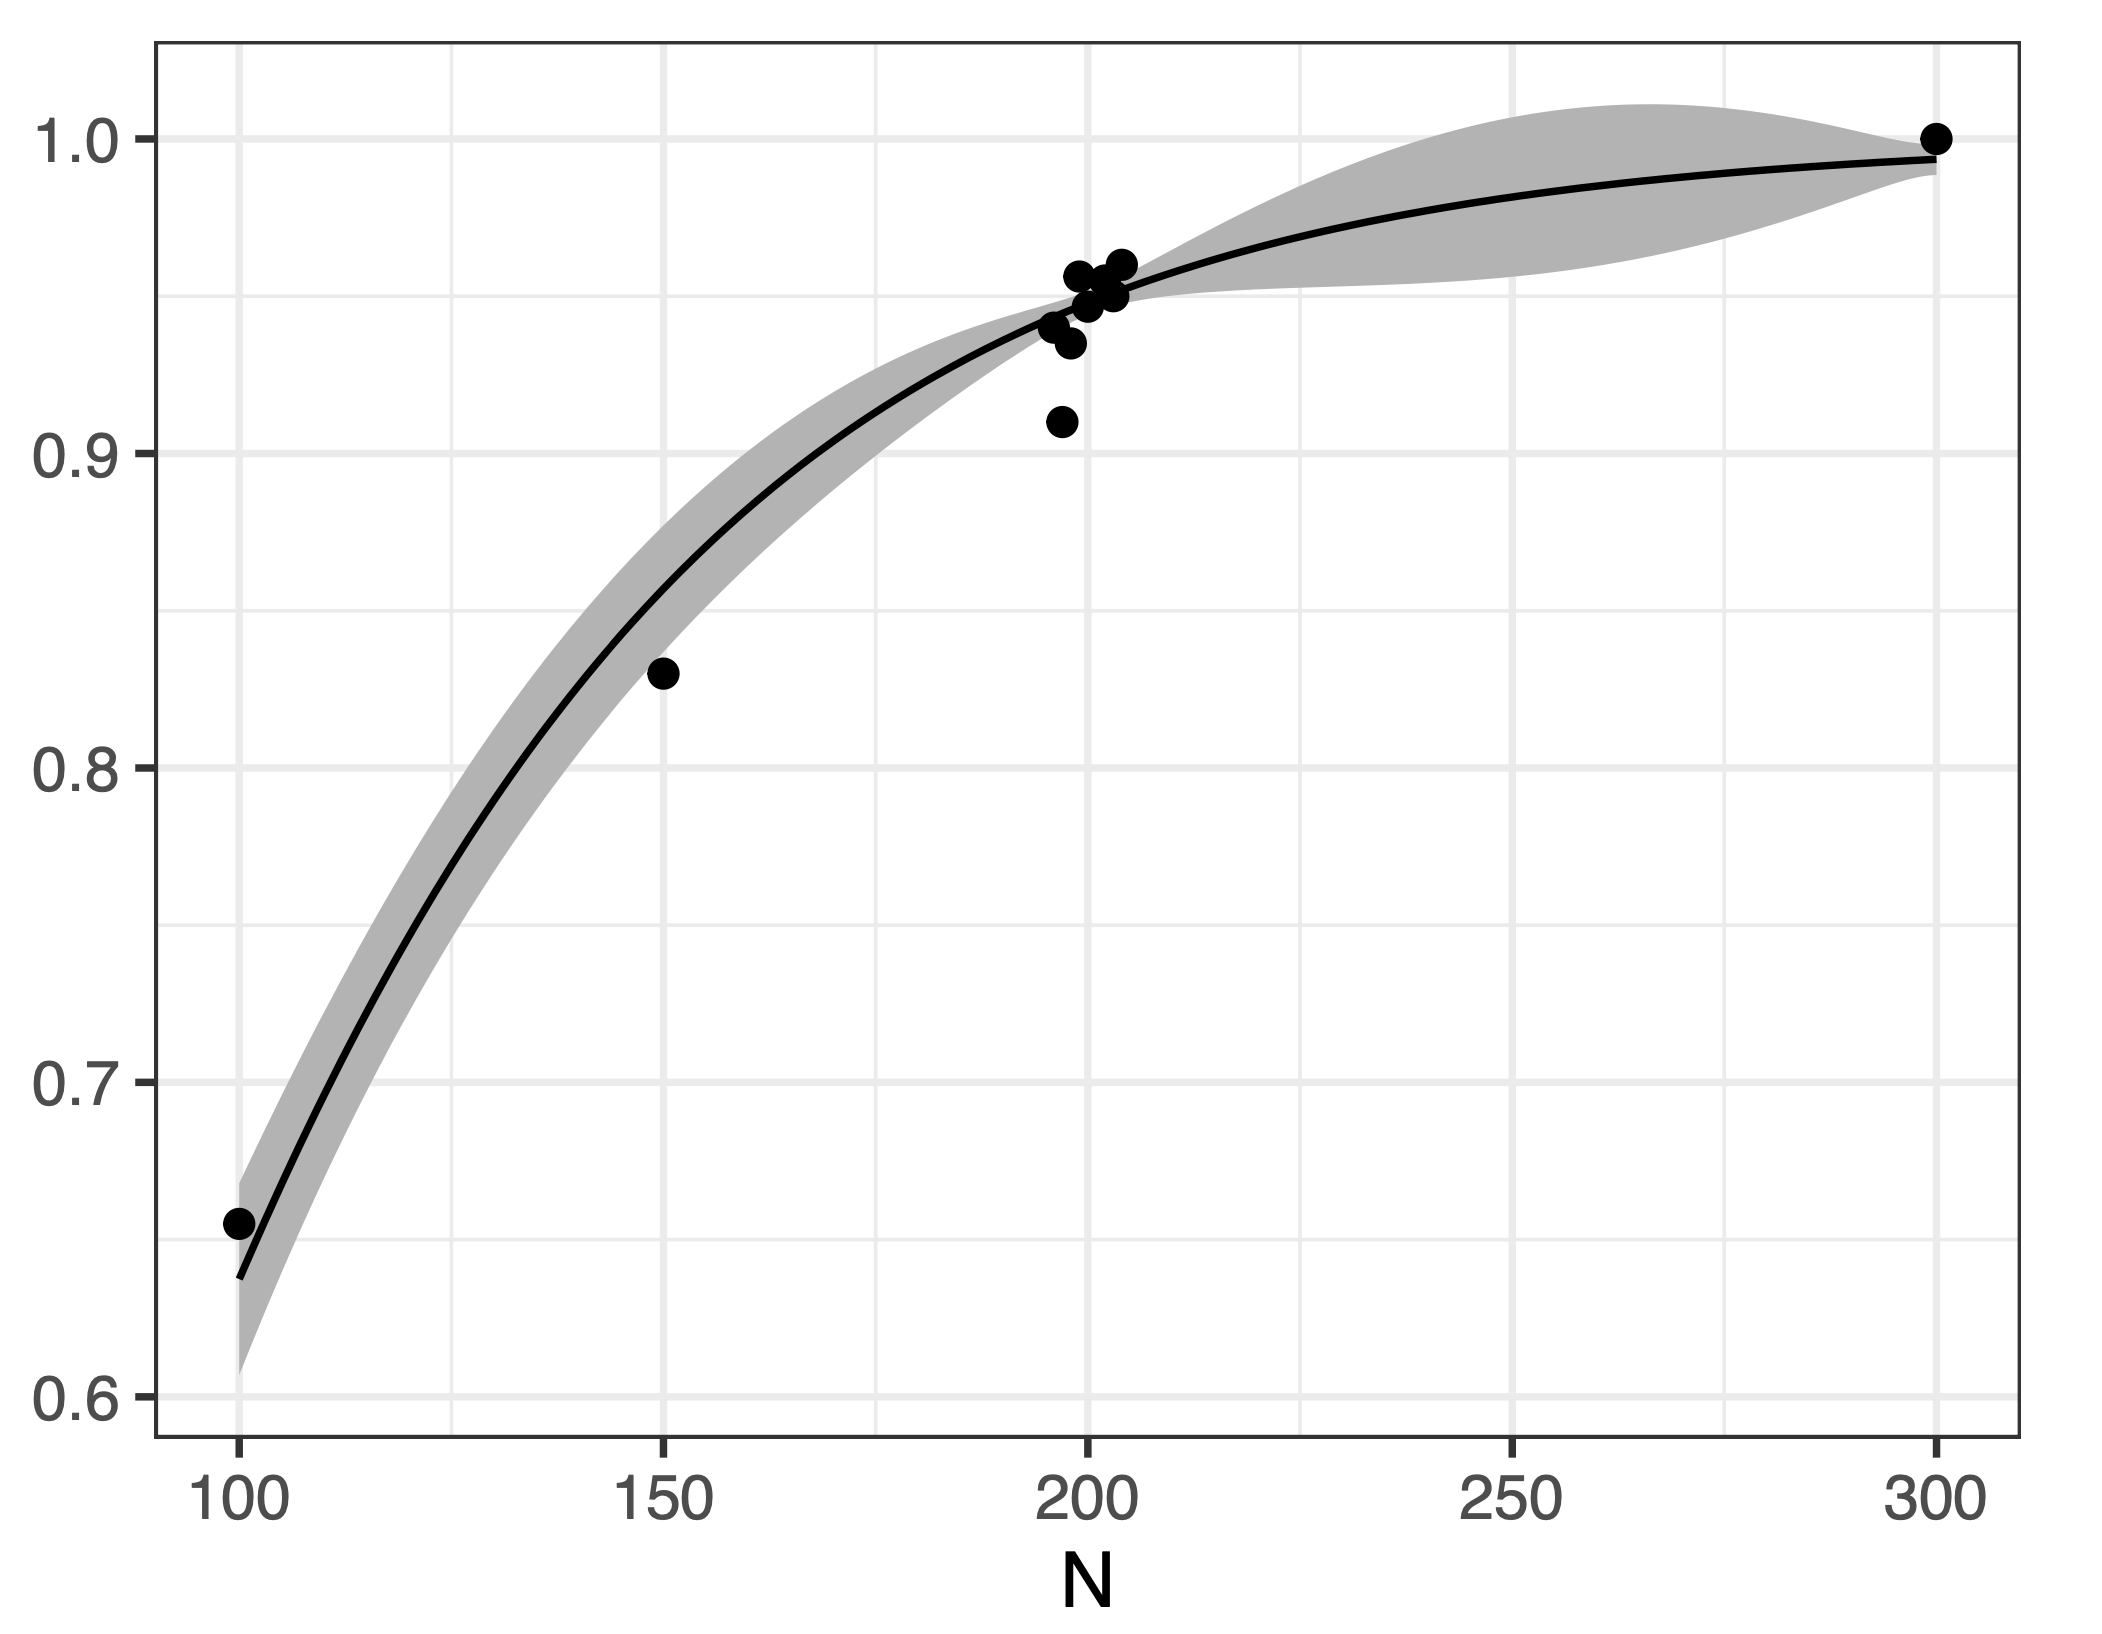
\includegraphics[width=\textwidth]{figures/mlpwr_example.png}

\end{frame}

\begin{frame}[t]{Slide explaining how we calculate the final sample size}

	\begin{enumerate}
		\item User specifies input parameters
		      \begin{cbox}{KCLtealblue}{}
			      \begin{itemize}
				      \item The expected large sample performance of the
				            model.
				      \item The range of sample sizes over which to search.
				      \item The number of signal and noise parameters.
				      \item The expected outcome prevalence.
			      \end{itemize}
		      \end{cbox}
		\item Set data, model, and metric functions based on user input
		      \begin{cbox}{KCLtealblue}{}
			      \begin{itemize}
				      \item Use defaults, but can be specified (e.g.\
				            \texttt{model = ``lasso''}).
			      \end{itemize}
		      \end{cbox}

		\item Tune the data generating model
		\item Perform search
	\end{enumerate}

	\gap

	We then return the minimum sample that is within 10\% of expect large
	sample performance in 80\% of replications.

\end{frame}

\begin{frame}[t]{Example 1:\ Binary outcome, logistic regression }

\end{frame}

\begin{frame}[t]{Example 2:\ Linear outcome, XGBoost}

\end{frame}

\begin{frame}[t]{Development status}
	Package in development; functioning, but more testing needed.

	\begin{itemize}
		\item Follow
		      \href{https://fediscience.org/@ewan}{\textcolor{KCLseablue}{fediscience.org/@ewan}}
		      for updates.
		\item Or enter an email address at
		      \href{https://tinyurl.com/pmsims-announce}{\textcolor{KCLblue}{tinyurl.com/is-it-ready-yet}}
		      to get one email when a public release is available.
	\end{itemize}

\end{frame}
\begin{frame}[t]{What's next?}

\begin{cbox}{KCLtealblue}{1.\ Machine learning}{}

\end{tcolorbox}

\begin{cbox}{KCLpurple}{2.\ Longitudinal data}{}

\end{tcolorbox}

\begin{cbox}{KCLseablue}{3.\ Common data types}{}
    e.g., clinical, NLP, genetic.

\end{tcolorbox}

\begin{cbox}{KCLhotpink}{4.\ Performance}{}

\end{tcolorbox}

\end{frame}

% For presentation: for example, a data with ~20 params and prevalence of 0.2 achieved performance of 0.75 AUC, We can then use our package to calculate sample size and compare with pmsampsize, Then, we use the tuned data generator from LR and check what is the performance for LR-Lasso and min sample size. Then, same for XGBoost. Riley seemed to advocate that XGBoost would need manifold more than LR, so we can check ![](20_f.png)

% Do it for ridge regression
% Do it for ML algorithms
% Then point to a mixed model.


\section{Conclusion}

\begin{frame}
  Questions?
\end{frame}

\appendix

\begin{frame}[allowframebreaks]{References}
    \printbibliography
\end{frame}

\end{document}
